\section{Box}

\subsection*{Design Overview}
\begin{table}[h!]
\centering
\begin{tabular}{l|l}
\toprule
\textbf{Parameter} & \textbf{Specification} \\ \bottomrule
Base Material & \textcolor{orange}{Aluminum 6061} or \textcolor{orange}{gold-plated copper} \footnotemark \\
pedestal drill $\Delta$ & \textcolor{orange}{3.8mm} \\
\bottomrule
\end{tabular}
\end{table}
\footnotetext{need to review alternatives}

\subsection*{Design Checklist}

\begin{itemize}[label={$\square$}]
    \item mounting wings to connect to the refrigerator.
    \item Parasitic Control -- Minimize cavity modes and conductivity loss (\href{https://arxiv.org/abs/1906.05425}{arXiv:1906.05425}) 
    \item Tightness (the box should close the PCB from all sides).
    \item Anchoring to the refrigerator.
\end{itemize}
\begin{figure}[h]
    \centering
    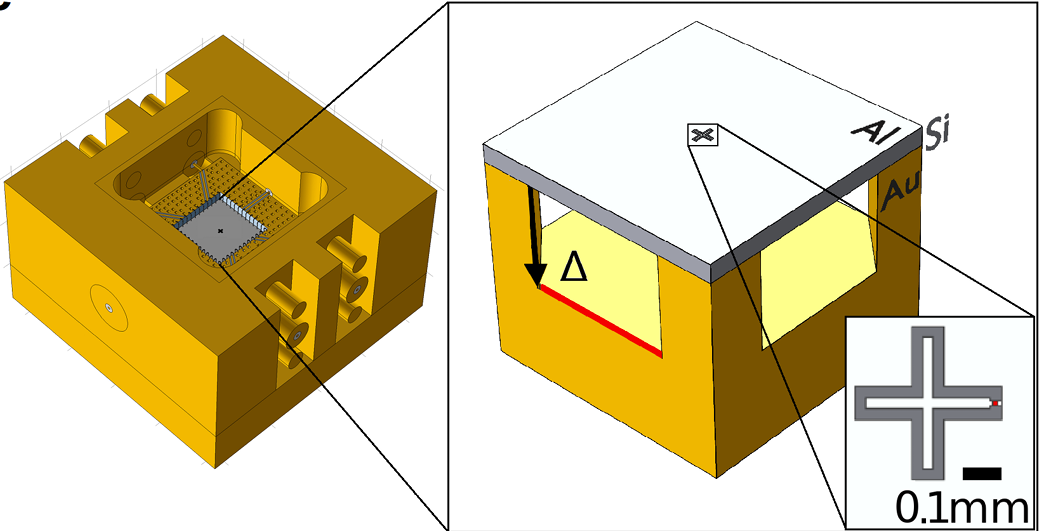
\includegraphics[width=0.6\linewidth]{tex/box example.png}
\end{figure}
